\documentclass[11pt,a5paper,oneside]{book}

\usepackage[
	top=1cm,
	bottom=1cm,
	left=1.5cm,
	right=2.5cm,
	headheight=17pt,
	includehead,includefoot,
	heightrounded,
]{geometry}

\usepackage[finnish]{babel}
\usepackage[utf8]{inputenc}
\usepackage[T1]{fontenc}

\title{Pion. P 32:n sotapäiväkirja (19826)}
% http://digi.narc.fi/digi/slistaus.ka?ay=80360

\usepackage{longtable}
\usepackage{setspace}
\usepackage{romannum}
\usepackage{graphicx}

\usepackage{hyperref}
\hypersetup{
    colorlinks=true,
    linkcolor=blue,
    filecolor=magenta,      
    urlcolor=blue,
}
\urlstyle{same}

\usepackage{xcolor}

\usepackage{changepage}
\usepackage{fancyhdr}
\usepackage{extramarks}
\pagestyle{fancy}
\fancypagestyle{headings}

%% L/C/R denote left/center/right header (or footer) elements
%% E/O denote even/odd pages

%% \leftmark, \rightmark are chapter/section headings generated by the 
%% book document class

%\fancyhead[C]{}
%\fancyhead[C]{\slshape Pion. P 32:n sotapäiväkirja}
\fancyhead[L]{}
\fancyhead[C]{Pion. P 32:n sotapäiväkirja 1941-1941 (19826)}
\fancyhead[R]{\firstxmark}
\fancyfoot[]{}
%\fancyhead[R]{\thepage}

\begin{document}

\extramarks{}{}

\begin{titlepage}
	\begin{center}
		\vspace*{1.5cm}
        \href{http://digi.narc.fi/digi/view.ka?kuid=3753911}{\Large Tulo 1264} \\
       	\vspace{1.5cm}
        \textbf{\Large Pion. P 32} \\
       	\vspace{1.5cm}
		\textbf{\Huge SOTAPÄIVÄKIRJA} \\
		\vspace{1.5cm}
		\Large 16.6.1941-17.10.1941 \\
   	\end{center}
\end{titlepage}

\extramarks{}{}
\section{Esipuhe}
Tämä sotapäiväkirja perustuu Kansallisarkiston digitaaliarkistosta löytyviin digitoituihin jaksoihin arkistoyksiköstä Pioneeripataljoona 32 1941-1941 (19826), joka löytyy osoitteesta: \\
\url{http://digi.narc.fi/digi/slistaus.ka?ay=80360} \\

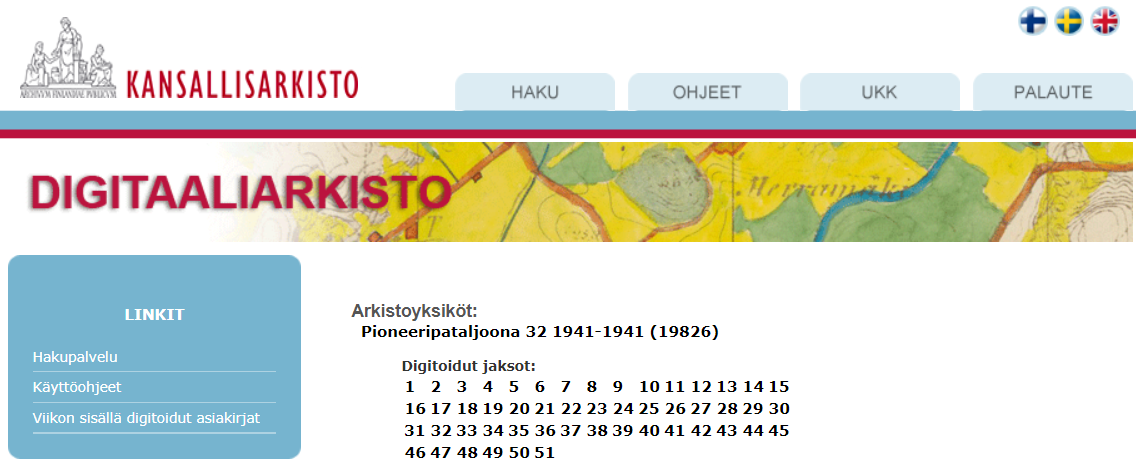
\includegraphics[scale=0.45]{jaksot_19826.png}

Kunkin sivun ylätunnisteessa oikeall on kyseisen digitoidun jakson numero ja linkki siihen kansallisarkiston digitoituun jaksoon.

Mikäli sotapäiväkirjan digitoidusta jaksossa on ollut vaikeuksia sanojen/merkintöjen tulkinnassa niin ne kohdat on merkitty \textcolor{red}{punaisella}. Linkki alkuperäiseen digitoituun jaksoon auttaa selvittämään näiden merkintöjen oikean merkityksen.

Sitä mukaa kun tekstissä on tullut lyhenteitä tai sanoja, joita lukija ei välttämättä tiedä niin näitä on pyritty selventämään sivun alalaidassa olevilla alaviitteillä. Lisäksi jokainen paikannimi on mainittu alaviitteissä helpottaakseen lukijaa seuraamaan etenemistä kartalta. Alaviitteissä saattaa löytyä myös muuta asiaan liittyvää lisäinformaatiota. Näitä alaviitteitä ei ole alkuperäisessä sotapäiväkirjassa.
%\FloatBarrier

\newcommand{\taulustart}[2]{
\newpage\extramarks{\href{#1}{#2}}{}
\begin{center} % optimoitu A5 formaattiin:
\renewcommand*{\arraystretch}{1.4}
\begin{longtable}{ | p{0.14\textwidth} | p{0.09\textwidth} | p{0.77\textwidth} |}
\hline \multicolumn{1}{|p{0.14\textwidth}|}{\textbf{Päiväys}} & \multicolumn{1}{p{0.09\textwidth}|}{\textbf{Kello}} & \multicolumn{1}{p{0.77\textwidth}|}{\textbf{SISÄLTÖ}} \\ \hline
\endfirsthead
\hline \multicolumn{1}{|p{0.14\textwidth}|}{\textbf{Päiväys}} & \multicolumn{1}{p{0.09\textwidth}|}{\textbf{Kello}} & \multicolumn{1}{p{0.77\textwidth}|}{\textbf{SISÄLTÖ}} \\ \hline
\endhead \hline \endfoot \hline \endlastfoot}

\newcommand{\taulustop}{\hline \end{longtable} \end{center} \newpage}

\taulustart{http://digi.narc.fi/digi/view.ka?kuid=3753912}{2}

16.6.41 & 11.00 & Kokoontuminen Lohjan Kauppalan Yhteiskoululla\footnote{Suurlohjankatu 2, Lohja}. Perustamispaikka ei ollut sopiva. Kun pataljoonan muodostavat reserviläiset olivat etupäässä lohjalaisia oli järjestyksen ylläpitäminen vaikeanlainen. Lisäksi vaikeutti perustamistapaikaksi valittu Yhteiskoulun pienuus järjestyksen ylläpitämistä. \\
% Lohjan Kauppalan Yhteiskoulu toimi aluksi vuokralla Anttilan talon vanhassa asuinrakennuksessa osoitteessa Suurlohjankatu 2, Lohja.

17.6.41 & 19.30 & Lähtivät kapt. Marrasmaa, luutn. Raimoranta, vänr. Helanto ja \textcolor{red}{ajomies} henkilöautolla Grabbskog träskiin\footnote{Grabbskog Storträsket, Raasepori} käskyn mukaisella tiedustelumatkalla yhteysottoon HR\footnote{Hangon Ryhmä}:ään.\\
% Träsk on ruotsia ja se on suomeksi järvi. Kartasta löytyy Grabbskog Storträsket Raaseporin läheisyydestä.

17.6.41 & 11.00 & Yksikköjen tuntolevyluettelot, ylimääräiset A- ja lääk. kortit lähetettiin SA-käskun mukaan Lohjan sk. toimistoon. Samoin luettelot puuttuvista korteista. 3 komppannian jako suoritettiin loppuun. Edelleen määrättiin lopullisesti kunkin yksikön päälliköt ja esikunnan kokoon- \\
\newpage

& & pano: Patalj. kom. Kapt. Marrasmaa,\newline adj. luutn. A. Gustafsson \newline pion. ups. luutn. I. Laatinen\newline talousups. luutn. S. Kärki \newline Autoups. luutn. J. Brax \newline 1.K.pääll. Ins. Kapt. Hotinen \newline 2.K.pääll. luutn. Korhonen \newline 3.K.pääll. luutn. Raimoranta \newline Valonheitinj. johtajaksi määrättiin vääpeli Huhtanen. \newline Raimorannan kompp. muodosti 13. Prikaatin pion. Komppaniat.\\

& 12.00 & Alkoi keskitysmarssi. Autorivistö lähti 12.07, johon kuului Esik., Valonheitinj. ja 2 K. johtajana luutn. Laatinen. \\

& 15.00 & Esik. ja 2 K-/ auto saapui Grabbskogträskiin. \\

& 16.15 & Lähetettiin 5 km auton hakemaan 1 K:aa \\

19.6.41 & 2.00 & Saapui 1 K:n miehet Leksvalliin\footnote{Leksvall, Raasepori}. \\

& 7.30 & Hevoset saapuvat Grabbskogträskiin. \\

& 7.45 & Ensimmäinen valm. ilmoitus. \newline $a=\frac{137}{19}$, $b=\frac{84}{82}$, $e=\frac{92}{424}$, $d=\frac{92}{532}$ \\
\taulustop

\taulustart{http://digi.narc.fi/digi/view.ka?kuid=3753913}{3}

19.6. & 9.15 & 3 Komppanian au-jaettiin, 5 au 1 K:aan ja 3 2:aan. \\

19.6-20.6 & & Majoitusjärjestelyjä. Ei mitään erikoista. 1 H-auto, 1 \textcolor{red}{ku}-auto ja 1 mp lisää Lohjalta. Esikunnan joukot epäkunnossa. Korjattu iltaan mennessä. 1 K:n pääll. Kapteeni Hotinen siirrettiin HR:n \textcolor{red}{Tukikohtaan}. Samoin vänr. \textcolor{red}{Ilomin} ja Koivula. Edellämainittu Pion. toimistoon. \newline 1 Kompp. ollut miinoitustyössä \newline 2 Kompp. järjestynyt majoitukseen ja osa ollut tietyössä\\ 

21.6. & 7.00 & Vaun. maitoa \newline Kävin DE:ssä, Maj. Laakso antoi määräyksen ruuhikaluston\footnote{\url{https://elavamuisti.fi/aikajana/ruuhikaluston-kaytto}} kuntoon laittamisesta. En vieläkään saanut karttoja. Meidän on itse koulutettava erikoismiehistömme. Osa Pion. kalustosta siirrettiin Pion. Tp:hen. \underline{\textcolor{red}{Kanttiini}} valmistui. 11 miestä siirrettiin 3 K:sta 2 K:hon.\\

22.6. & 7.00 & valm. ilm. $a=137, b=87, e=102, d=100$ \\
\newpage
& 7.00 & Ilmoitukset \%:ssa kokovahvuudesta = 100\%, autovahvuus 31 \%, hevosvahvuus 100 \%.\\ 

& 16.10 & \underline{Pion. Kom. kirje 31}/Pion./\Romannum{2}/F/sal. Kompp. \newline Koulutuksesta: 11. ja 2 K noudatettava yleistä kertausharjoituskoulutusohjeita. 3 K:n koulutuksen painopiste tulee olla rynnäkköpion. koulutuksessa siten, että \textcolor{red}{u} joukkue pystyy väkivaltaiseen ylimenoon.\newline Pataljoonan on suoritettava tiedustelua mahdollista ylimenoa varten peitepiirroksessa mainitulla linjalla 1/A-B ja ryhdyttävä valmistamaan uivaa siltaa kohdassa L (Solböle\footnote{Solböle, Raasepori}) \newline Kirje 32/Tietetio/\Romannum{3}/sal. mukaan on patalj. ryhdyttävä tientekoon alkaen A:sta ja huomioimattaan sen, ettei muu pion. koulutus kärsi. Tie tehtävä yhteen suuntaan liikennöitäväksi autotieksi \textcolor{red}{sivuuten kohteisiin.} \\

23.6. & & Yhteys JR 55:en everstil. Wiberg. Keskusteltiin tien A-B rakentamisesta. Pyydettiin apua. Ei tule? \\

\taulustop

\taulustart{http://digi.narc.fi/digi/view.ka?kuid=3753914}{4}

23.6. & & Ilmoitettu komppanioille hälytysvalmiudesta. Vänr. \textcolor{red}{Sjöblom} 2 au pat. \textcolor{red}{Haastaman} käyttöön. \\

& 18.00 & valm. ilm. $a=131, b=89, e=103, d=132$ \newline valm. ilm. 1) 102, 2) 49, 3) 100. \\

24.6. & & Valm. ilm. sama kuin ennen\newline 3 K. alistettu muualle.\newline Saatu uusia tehtäviä:\newline 1 K \underline{Miinakenttää} ei saa rakentaa lisää.\newline Radan korjausvälineet otettiin pois Skogbyhyn\footnote{Skogby, Raasepori} saakka. Skogby-järven ympäri tehtiin tie. Lehvallin laiturin viimeistely. Rautatien \textcolor{red}{poly} puolella oleva rataylimenopaikat valmistetaan.\newline \underline{Oikotie} tehtävä Österbyssä\footnote{Österby, Raasepori}.\newline \underline{2 K.} Huoltotie PAp:n luota etelään.\newline Lautan siirtäminen \textcolor{red}{Åminneforssin}\footnote{Åminnefors, Raasepori} padon alapuolelta yläpuolelle.\newline Solbölen ylikulkupaikka järjestettävä lautoilla. 2 lauttaa.\newline Saatu määräys maastl. ajoneuv. maalauksesta. \\

25.6. & & Palvelusohje no 1 saatu.\newline Valm. ilm. tavalliseen tapaan. Ei mitään erikoista. 2 K. siirtyi Troll-\\
\newpage
& & shovdaan\footnote{Trollshovda, Raasepori}. Lautan siirtäminen vaikeaa. Rakennetaan uusi lautta \textcolor{red}{kansineen työvälineillä}. \\

26.6. & & Patalj. sai kirjallisen tiedoituksen huoltotien loppuun rakentamisen siirymisestä JR 55:lle. Lautta valmis. \\

27.6. & & Saaru HR:n käsky no 1 kenttäröistä. Tehtiin henkilöstötäydennys: 1 \textcolor{red}{ueäk} au + 5 mekaanikkoa; 10 autonkulj. + 1 autonasentaja + 1 käsityöläinen.\newline Valm. ilm. tavalliseen tapaan. \\

28.6. & & Ei mitään erikoista. Kaiken aikaa jatkettu yleensä varustus- ja työvälineiden tasausta. Autojen täydennys ja huolto jatkuvasti heikkoa. Pataljoonan kuorma-autoista saatu ainoastaan 50\%. \\

29.6. & & Solbölen kumpikin lautta valmistui liikennekelpoisiksi. Koekuormitettu (8 tonnin kuorma) \\

30.6. & 6.30 & Pion. kom. määräyksestä 1 pion. ryhmä ups. \textcolor{red}{puolella} alistettiin Maj. Lagerlöfiin, \textcolor{red}{Armeijassa}.\newline Vänr. Murtomäki määrättiin johtajaksi. Tehtävänä raivata ryssien jättämä Horsön\footnote{Horsön, Raasepori} saari\\

\taulustop

\taulustart{http://digi.narc.fi/digi/view.ka?kuid=3753915}{5}

& & miinoituksista ja ansoituksista. \\
& 9.20 & Ryhmä lähti.\newline 2 K. pääosa palasi Solbölestä.\newline Kirjallinen valm. ilmoitus.\\

1.7.41 & & Solbölen asia selvä. Henkilösiirtoja toimitettu. 38 LK:aan siirretty 2 miestä; Kev.Os 19:ään 1+9 miestä.\\

& 20.30 & Murtomäen ryhmä palasi. Ei mitään erikoista.\newline Valm. ilm. tavalliseen tapaan.\newline 3 K., joka on alistettu muualle pataljoonan tuntemattomaan tehtävään, ei pysty tällä kertaa antamaan asianmukaista tilanneilmoituksia.\\

\newpage

2.7.41 & 10.00 & Ilmoittautui ev.ltn. 7. Ch. Fabritius. \newline Komentaja ja ev.ltn. F. seurasivat 2. K:n koulutusta aamupäiväläl. Iltapäivällä tilauksen esiesittely ev.ltn. Fabritiukselle. \\
& 19.05 & Osui yksi ryssän järeän tykistön ammus 40 m:n päähän Österbyn\footnote{Österby, Raasepori} sk-talosta, josssa majaili 1/3 K. Aineelliset vahingot hyvin pienet.\newline Ei haavoittuneita. \\

3.7.41 & & Tasoituksia ja siirtoja 3 K. luovuttu 3 kuormallista kelvotonta materiaalia, rikkinisiä \textcolor{red}{ivt}. varusteita u. m. Pataljoona puolestaan luovuttanut ETp:hen ylimääräistä ja rikkinäistä materiaalia.\newline Koulutukset jatkuvat.\\

\taulustop

%\FloatBarrier
%\newpage

\end{document}